\section{Quantification}

As mentioned in \cref{sec:crna_quantification}, all the \gls{bsj} detection
tools also quantify the number of reads supporting each \gls{bsj}.
However, there are several tools that focus on the quantification of
\gls{crna}s based on previously detected \gls{bsj}s.
nf-core/circrna offers two such tools: CIRIquant and psirc-quant.

Due to the lack of a ground truth or a gold standard, the quantification
results were compared to each other.
The correlation heatmaps in \cref{fig:correlation_heatmap} show the Pearson
correlation coefficient between the quantification results of the detection
tools, multiple aggregations of the detection tools, and the quantification
tools.

\begin{figure}[ht]
    \begin{tabular}{cc}
        \begin{subfigure}{0.5\textwidth}
            \centering

            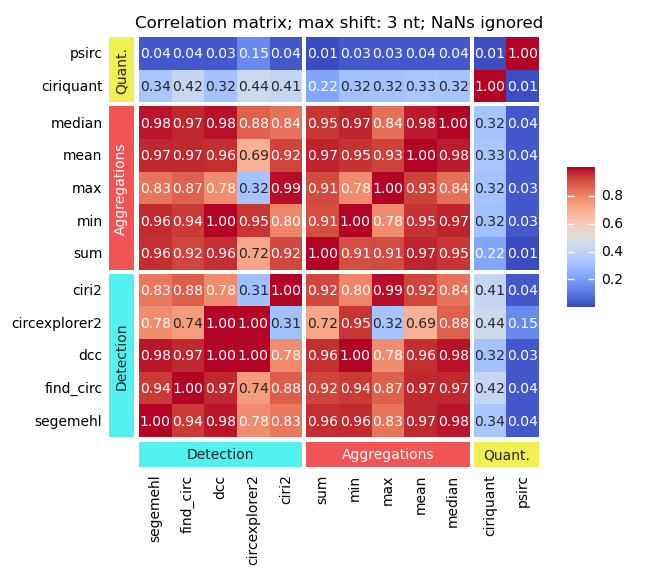
\includegraphics[width=\linewidth]{chapters/4_results_and_discussion/figures/quantification/correlation_heatmap_3_na.png}
            \caption{Missing values treated as NaN}
            \label{fig:correlation_heatmap_3_na}
        \end{subfigure}
         &
        \begin{subfigure}{0.5\textwidth}
            \centering

            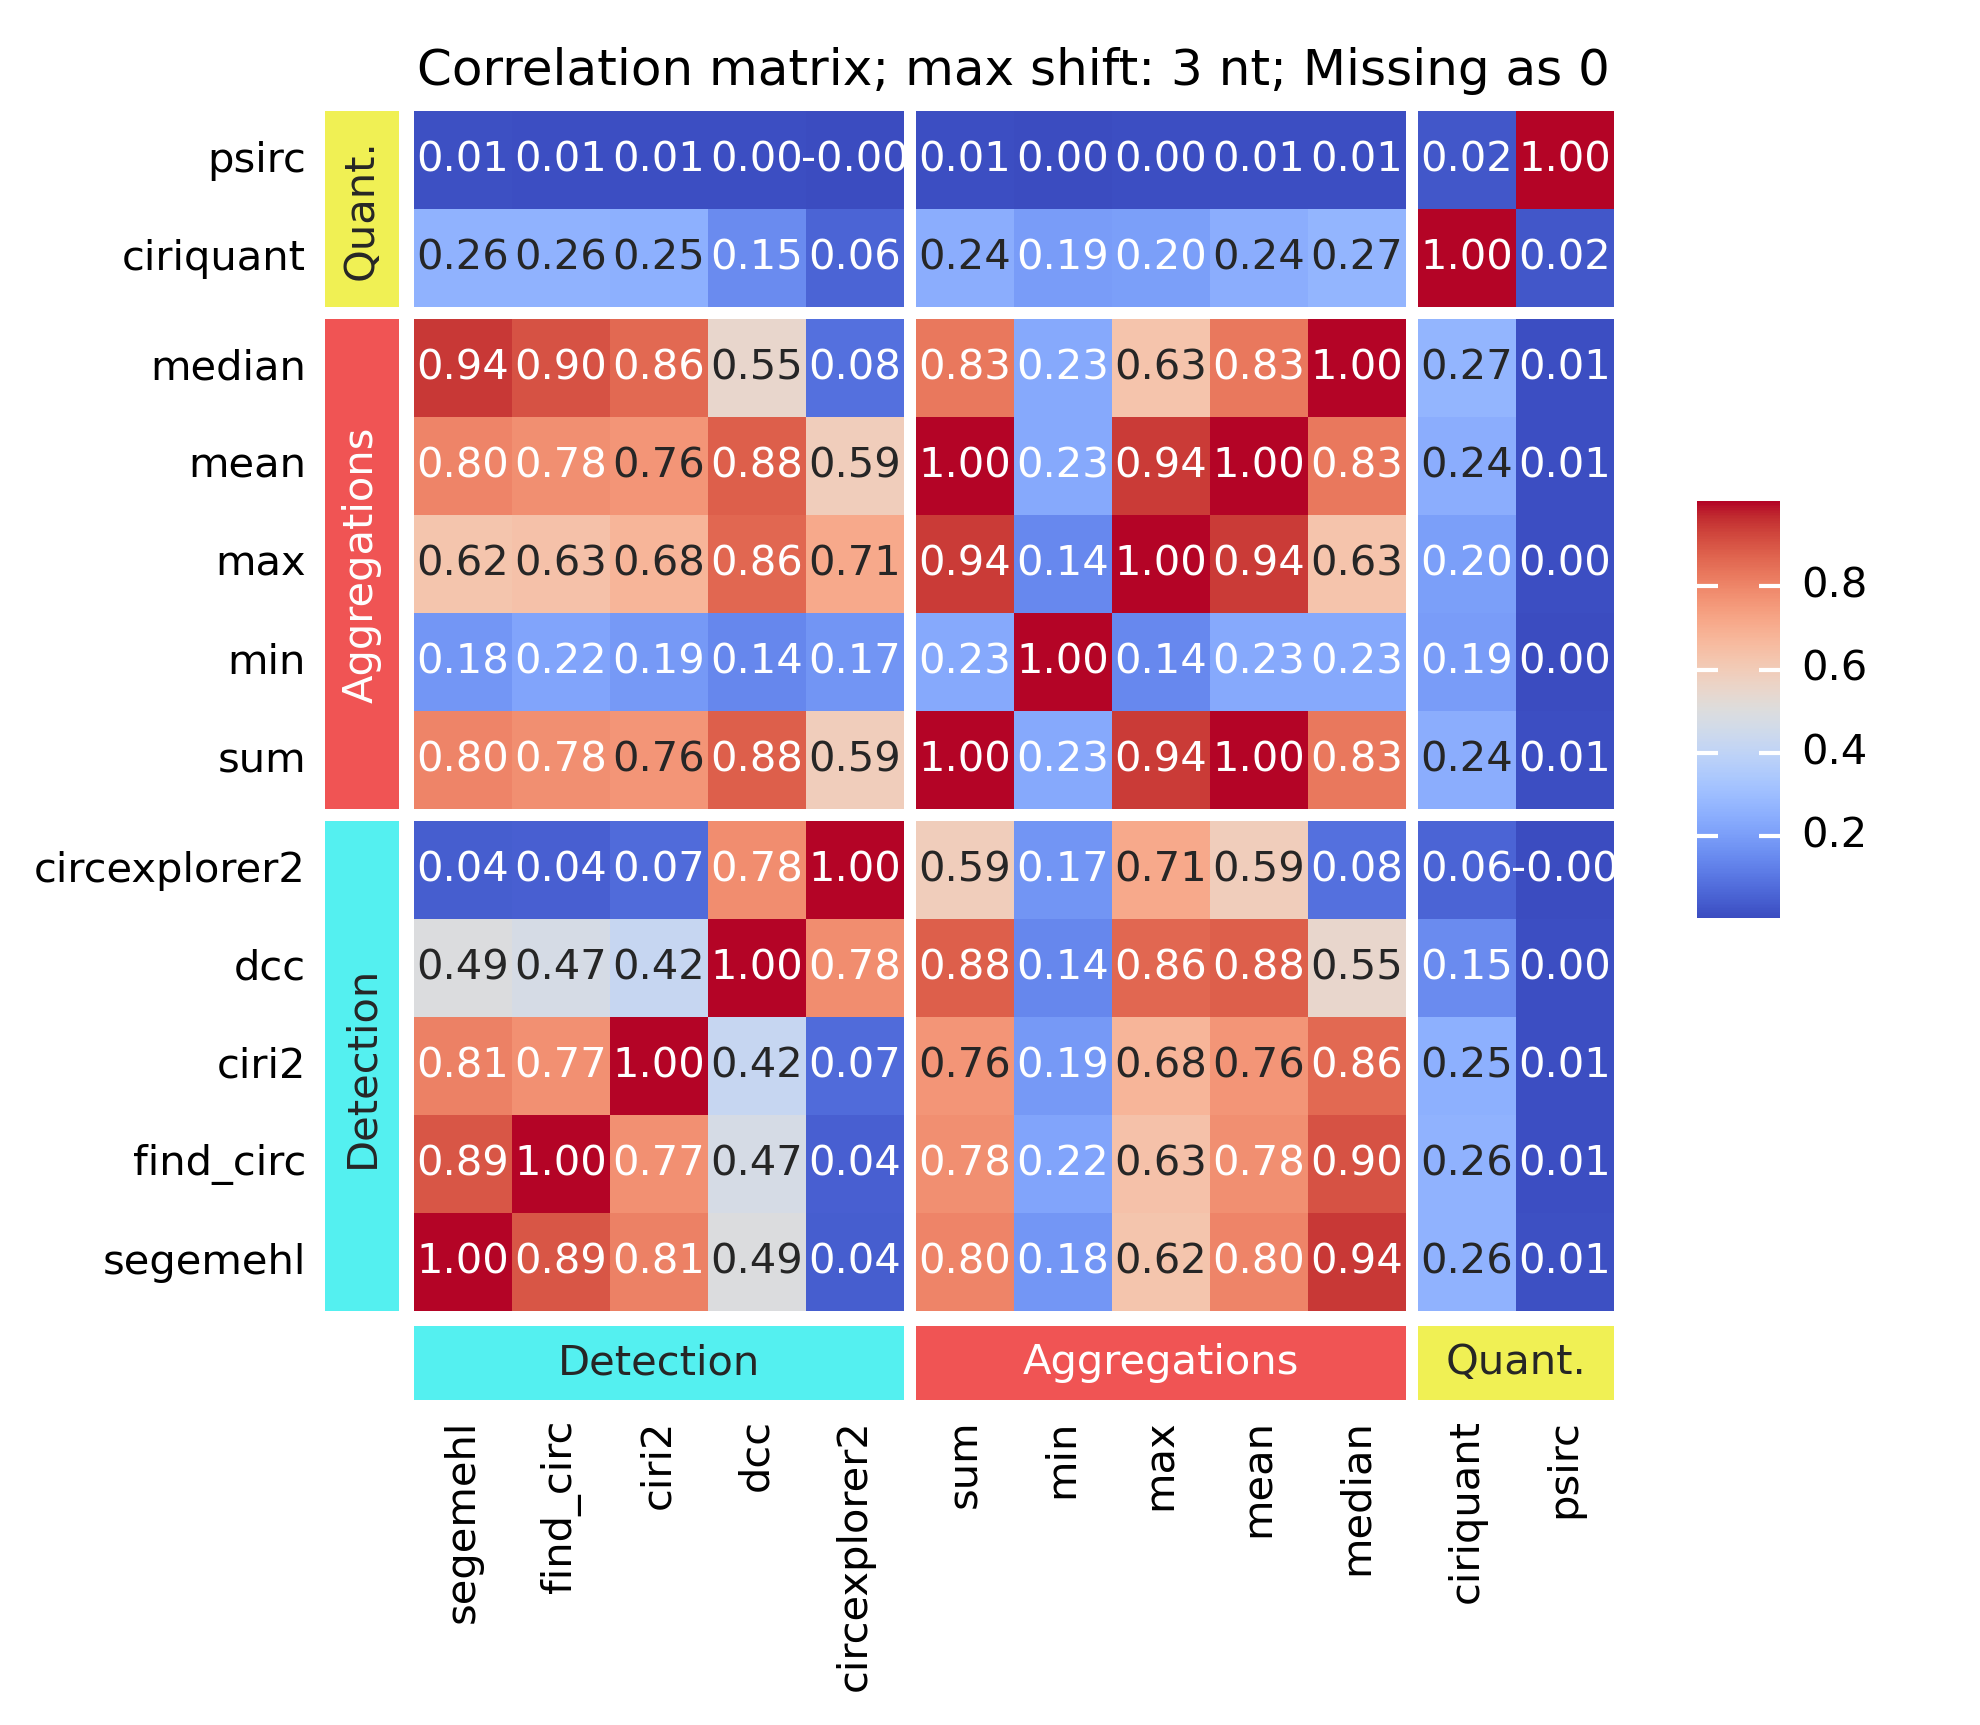
\includegraphics[width=\linewidth]{chapters/4_results_and_discussion/figures/quantification/correlation_heatmap_3_0.png}
            \caption{Missing values treated as 0}
            \label{fig:correlation_heatmap_3_0}
        \end{subfigure}
    \end{tabular}
    \caption{Pearson correlation heatmap between the quantification results of
        the detection tools, multiple aggregations of the detection tools, and
        the quantification tools.
        The expression values were scaled so that the sum per sample and tool was
        constant.
        For each detected \gls{bsj}, expression information of all \gls{bsj}s within a
        \textit{max shift} of 3 was summed.
        While treating missing values as NaN results in higher correlations overall,
        treating the zeros as actual 0 values better reflects the underlying data.
        This is because missing values mean that a tool did not detect any reads
        supporting a \gls{bsj} (thus not outputting anything), which is equal to the
        definition of 0 expression.
        In \cref{fig:correlation_heatmap_3_0}, we can see that the quantification tools
        show relatively low correlation with the detection tools and aggregations.
    } \label{fig:correlation_heatmap} \end{figure}

\subsection{Quantification tools}
Interestingly, the quantification tools show relatively low correlation with
the detection tools and aggregations.
While both show robust results in their respective publications, they were only
tested on paired end data\supercite{zhang_accurate_2020,yu_quantifying_2021}.

\paragraph{psirc}
For psirc, there is an additional complication: As mentioned in
\cref{sec:psirc}, it expects the full-length isoform \gls{crna}sequence as
input.
As we only have single-end data, we cannot provide this information.
Therefor, the entire sequence within the \gls{bsj} boundaries is used as the
\gls{crna} sequence.
While psirc uses the information that the sequence is circular when
constructing the Transcript de Bruijn Graph (T-DBG), it does not treat reads
spanning the \gls{bsj} differently from reads that do
not\supercite{yu_quantifying_2021}.

While due to the lack of ground truth it is impossible to say that the
quantification results of psirc are wrong, the low correlation with the
detection tools indicates that they are at least questionable in this context.
Thus, I will not use the quantification results of psirc in the following
analyses.

\paragraph{CIRIquant}
CIRIquant, on the other hand, shows a higher correlation with the detection
tools and aggregations.
However, it is still relatively low (< 0.3 in all comparisons when treating
missing values as 0).
